\section{Chosen Solution}
To provide the project with valuable information about how the system could work in the real world, we will also choose a solution for the hardware elements.
This is despite the fact that only the chosen software solution, that is the website, the API, and some simulated hardware elements.

For the availability of bicycles, we choose to have docks since it also covers part of the hardware aspect of a different requirement, remote locking.  
For remote locking we also choose to use passwords that need to be input at the station because it is something everyone can do once the booking has been done, as SMS, QR codes, and GPS require phones and might not be suitable for tourists.
If it comes to tracking of bicycles we choose GPS because it requires less equipment than WiFi to implement.

The following provides an overview of the chosen solution using rich pictures.

The server-station relationship is shown in \figref{fig:ServerRichPicture}.
It depicts a central server, where the different bicycle stations are connected to it.
Furthermore, people can access the server to gain information e.g. bicycle count, but also to register bookings to the server, which will then communicate this to the given station(s)
The stations also have the capability of handling booking by themselves, which is then shared with the central server..
The server contains collected information from each station, such as bookings, amount of available bicycles at stations, and usage statistics.
It provides booking and amount of available bicycles at stations through a website to the user. 
Usage statistics are provided to the facilitators of the system and gives them the ability to improve it. 

\begin{figure}[h]
\centering
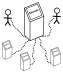
\includegraphics[scale=3]{serverrichpicture/server.pdf}
\caption{The server and the associated stations.}
\label{fig:ServerRichPicture}
\end{figure}

The dock that provide the locking/unlocking mechanism along with the bicycle detection ability have to talk to the station. 
This is for example when they need to unlock booked bicycle, the information needs to be propagated from the server to the station to the individual bicycle.
This can be seen in \figref{fig:StationRichPicture}.
The figure depicts a station and two docks connected to the station, which contains a bicycle each. 
On the display of the station, it can be seen that two bicycles are available for use.
This is a sketch of how a station could look like when deployed.
\begin{figure}[h]
\centering
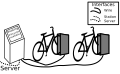
\includegraphics[scale=3]{stationrichpicture/station.pdf}
\caption{The station and the bikes.}
\label{fig:StationRichPicture}
\end{figure}